\chapter{Monte Carlo Methods \& RBM}

We were assuming that by using apriori knowledge it was possible to draw a graph highlighting the dependencies among all the variables in the problem. But in a real world application what we have is data. Therefore in order to learn about the dependencies we can use data in two different ways.

\begin{itemize}
    \item Learning the graph structure. We can use data to induce the structure of the graph. This is simply done by performing an iterative search among the different possible graph topologies. Once you have the structure you can use the data to estimate the conditional distribution probability associated to each node.

    \item Use latent variables. In deep learning instead of trying to understand the relation or dependencies among variables, you make the assumption that there are hidden variables that you cannot observe. Therefore, we will observe a subset of the total variables called visible variables which will have a connection to the hidden or latent variables. The weights of these connections will describe if the interaction of a certain visible variable $v_i$ is strong with another hidden variable $h_i$. This computation will be less computational extensive than trying to learn the correct graph topology for the visible variables. Finally, this model can be trained using gradient descent.
\end{itemize}

%Inferring the marginal probability distributions over some nodes or the conditional probability distribution of some nodes given other nodes is computationally extremely costly. As a result deep learning usually relies on making a good enough inference approximation.

\section{Example: Shallow Restricted Boltzmann Network}
An example of using latent variables for approximating the dependencies among a set of random variables is the Restricted Boltzmann Machine Network. This model uses binary units and two sets of variables: visible variables $v_i$ and hidden or latent variables $h_i$. The goal of the model is to estimate the joint probability of all the variables combined.

\noindent The visible variables are not connected to each other and the same is true for the latent variables. The visible variables will be connected to all latent ones and vice-versa. This is done in order to simplify the estimation of the conditional probability. With this architecture, $P(h | v)$ and $P(v | h)$ are factorial and easy to compute. 

\begin{figure}[h]
    \centering
    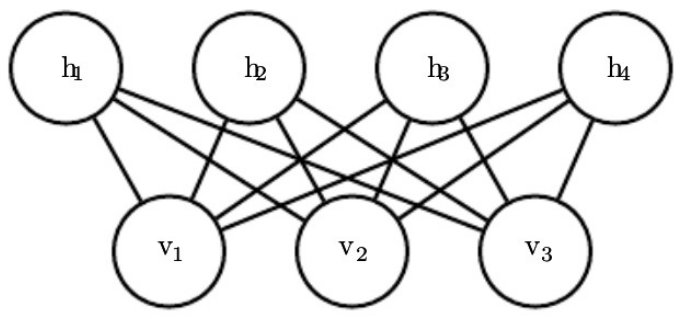
\includegraphics[width=7.5cm]{Images/rbm.jpg}
    \caption{Architecture of a Restricted Boltzmann Machine}
\end{figure}

\noindent The Restricted Boltzmann Machine is an energy based undirected model. Therefore the joint probability $P(v, h)$ can be described as:

$$ P(v, h) = \frac{1}{Z} \exp{\left( -E \left(v, h\right) \right)} $$

\noindent Where the energy function $E(v, h)$ is:

$$ E(v, h) = -b^{T}v -c^{T}h -v^{T}W h $$

where $W$ is the weight matrix of the connections between $v_i$ and $h_i$, $b$ is the bias of the visible units and $c$ is the bias of the latent units.

\noindent Meanwhile the partition function $Z$ is:

$$ Z = \sum_v \sum_h \exp \left( -E(v, h)  \right) $$

\noindent We can prove why calculating the posteriori probabilities $P(v|h)$ and $P(h|v)$ is tractable from a computational point of view (we know that doing the same for $P(v)$ is not, computing $P(v)$ will involve summing over all possible configurations of the visible units).

$$ P(h | v) = \frac{P(h, v)}{P(v)} = \frac{1}{P(v)} \frac{1}{Z} \exp \left( b^{T}v + c^{T}h + v^{T}W h  \right) $$

\noindent Because we can observe the visible variables $v_i$ the probability $P(v)$ will be a constant, the same is true for $b^Tv$ we can rewrite the partition function $Z$ as $Z'$.

$$ P(h | v) = \frac{1}{Z'} \exp \left(c^{T}h + v^{T}W h  \right) $$

\noindent Now due to not having connections between the hidden variables we can rewrite the equation making explicit the contribution of each variable.

$$ P(h | v) = \frac{1}{Z'} \exp{ \left( \sum_{j=1}^{n_h} c_j h_j + \sum_{j=1}^{n_h} v^{T} W_{: j} h_j  \right)} $$

\noindent Which can also be rewrite it as:

$$  P(h | v) = \frac{1}{Z'} \prod_{j=1}^{n_h} \exp \left( c_j h_j + v^{T} W_{: j} h_j  \right)  $$

\noindent Finally by using $\sigma(x) = \frac{\exp{(x)}}{1 + \exp{(x)}}$ and $1 - \sigma(x) = \sigma(-x)$, the unnormalized probability can be written as:

$$ \Hat{P} (h | v) = \prod_{j=1}^{n_h}  \sigma \left( \left( 2h -1 \right) \odot \left( c + W^T v \right) \right)_j $$

\noindent and with a similar derivation:

$$ \Hat{P} (v | h) = \prod_{j=1}^{n_v}  \sigma \left( \left( 2v -1 \right) \odot \left( b + W h \right) \right)_i $$

\newpage
\noindent During training given training data $x$ to be represented in the visible units, we will have to maximize the log-likelihood $log(p(x, \theta))$. The gradient with respect to $\theta$ is

$$\nabla_{\theta}~ log \left(p(x, \theta)\right) = \nabla_{\theta}~ log \left(\Hat{p}(x, \theta)\right) - \nabla_{\theta}~  log \left(Z (\theta)\right) $$

\noindent Computing the first term is not a problem for Restricted Boltzmann Machines however the second term is more problematic as is not possible to compute exactly but we will be able using MonteCarlo methods to compute a good approximation of it.


\section{Monte Carlo Method}

Monte Carlo sampling is a randomized algorithm that is used to estimate a sum or an integral using random generated samples. The idea is to view the sum or integral as if it was an expectation under some distribution and to approximate the expectation by a corresponding average.

$$ s = \sum_{x} p(x)f(x) = \mathbb{E_{p}} \left[ f(x) \right] ~~~~ s = \int {p(x)f(x)dx} = \mathbb{E_{p}} \left[ f(x) \right] $$

\noindent We can approximate $s$ by drawing $n$ samples $x^{(1)} ,..., x^{(n)}$ from $p$ and then forming the empirical
average.

$$ \hat{s}_n = \frac{1}{n} \sum_{i=1}^{n} {f(x^{(i)})}  $$

\noindent Keep in mind that the number of random samples we have to generate to have a good approximation is usually large ($\sim 10^4 - 10^6$ samples). However, all this relies on our ability to easily sample from the base distribution $p(x)$.

\section{Importance Sampling}

Since sampling from $p(x)$ is not always possible, we can rearrange which part of the integrand should play the role of the probability $p(x)$ and which should play the role of the function $f(x)$ to estimate. We can rewrite $p(x)f(x)$ as:

$$ p(x) f(x) = q(x) \frac{p(x)f(x)}{q(x)} $$

where we now sample from $q(x)$ and average on $ \frac{pf}{q} $

\noindent This may be useful if it is feasible to sample from $q$ but not from $p$. Also a good $q$ can reduce the
variance of the estimate. Now the minimum variance will occur when q is:

$$ q^{*} (x) = \frac{p(x) |f(x)|}{Z}$$

where $Z$ is the normalization constant, chosen so that $q^{*} (x)$ sums or integrates to 1 as appropriate. This is called the optimal importance sampling. Determining the optimal q requires solving the original integral so is not useful in practice.

\newpage
\section{Markov Chain}

Monte Carlo and importance sampling rely on the assumption that we can sample from $p$ or $q$ easily. This is only true when $p$ or $q$ have a directed graphical model representation (ancestral sampling). On the other hand, sampling from undirected models is more difficult. On those cases we will use the Markov Chain Monte Carlo method. The key idea behind it is to construct a Markov chain such that the distribution of samples over time converges to the desired target distribution.

\begin{figure}[h]
    \centering
    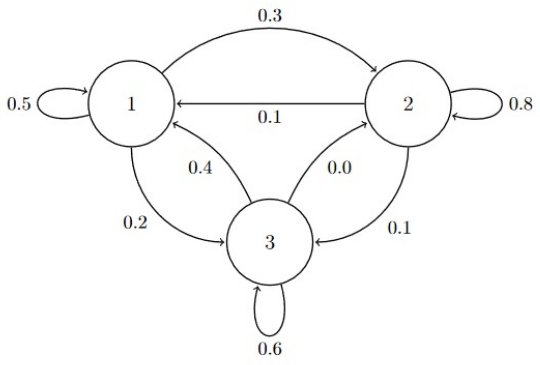
\includegraphics[width=5cm]{Images/markov-chain.jpg}
    \caption{Markov Chain example}
    \label{fig:markov-chain}
\end{figure}


\noindent A Markov chain represents a sequence of events where the probability of transitioning from one state to another depends only on the current state.

$$ P(X_{n+1}=x' \vert X_n = x) $$

\noindent This property is known as the Markov property or memory-less property. Formally, a Markov chain is defined by a random state $x$ and a transition distribution $T ( x' | x)$ specifying the probability that the state $x$ will change to the different possible states $x'$. Running the Markov chain means repeatedly updating the state $x$ to a state $x'$ sampled from $T(x'|x)$. The probability of landing in state $x'$ when we are in state $x$ is given by:

$$ q^{(t+1)} (x') = \sum_x q^{(t)} (x) T(x | x')  $$

where $q(x)$ represents the probability distribution of being in state $x$ at time $t$.


\subsection{Gibbs Sampling}

A conceptually simple and effective approach to building a Markov chain that samples from $p_{model}(x)$ is to use Gibbs sampling. Sampling from $T(x'|x)$ is accomplished by selecting one variable $x_i$ and sampling it from $p_{model}$
conditioned on its neighbors in the undirected graph. An example:

\begin{figure}[h]
    \centering
    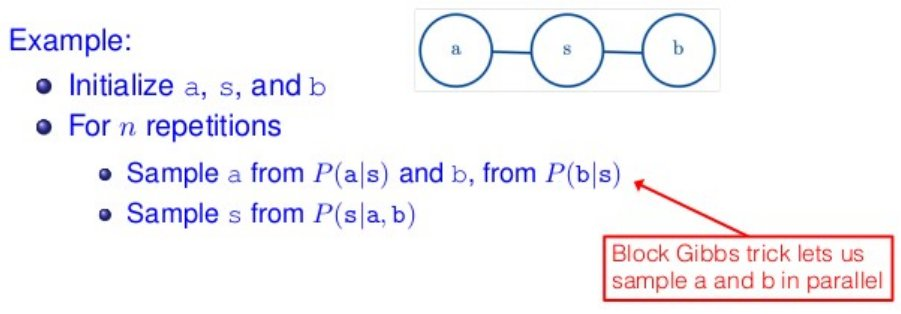
\includegraphics[width=10cm]{Images/gibbs-sampling.jpg}
    \caption{Gibbs sampling algorithm example}
    \label{fig:gibbs-sampling}
\end{figure}

It is also possible to sample several variables at the same time so long as they are conditionally independent given all of their neighbors. This is called block Gibbs sampling and is used in Restricted Boltzmann Machines.

\newpage

\section{Training Restricted Boltzmann Machines}

Now that we know bow to perform Gibbs sampling, we can train Restricted Boltzmann Machines. 

\noindent As usual we will train the network using the Maximum Likelihood Estimator. Therefore, given training data $T=\{ x^{(i)} \}_{i=1}^n$ we want to find the parameters $\theta = \{ W, b, c \}$ that maximize $ log \left( p(T | \theta) \right)$.

$$ log \left(p(T | \theta)\right) = log \left( \frac{1}{Z(\theta)} \Hat{p} (T | \theta)  \right) = log \left( \Hat{p} (T | \theta)  \right) - log \left( Z(\theta) \right)$$

\noindent where

$$ log \left( \Hat{p} (T | \theta)  \right) = log \left( \prod_{i=1}^n    \Hat{p} (x^{(i)} | \theta)  \right) = \sum_{i=1}^n log \left(    \Hat{p} (x^{(i)} | \theta)  \right) $$

\noindent Therefore we will proceed to compute the gradient ascent by computing:

$$ \nabla_{\theta}~ log \left(p(T | \theta)\right) = \sum_{i=1}^n \nabla_{\theta}~ log \left( \Hat{p} (x^{(i)} | \theta)  \right) - \nabla_{\theta}~  log \left( Z(\theta) \right)  $$

\noindent Operating on the first term we get the following:

$$ \sum_{i=1}^n \nabla_{\theta}~ log \left( \Hat{p} (x^{(i)} | \theta)  \right) = \sum_{i=1}^n \frac{1}{\Hat{p} (x^{(i)} | \theta)} \nabla_{\theta}~ \Hat{p} (x^{(i)} | \theta)   $$

\noindent Using the energy function and that $x^{(i)} = v^{(i)}$

$$ = \sum_{i=1}^n \frac{1}{\sum_h exp \left( -E (v^{(i)}, h) \right)} \nabla_{\theta}~ \sum_h exp \left( -E (v^{(i)}, h) \right) = - \sum_{i=1}^n \sum_h \frac{exp \left( -E (v^{(i)}, h) \right)}{\sum_h exp \left( -E (v^{(i)}, h) \right)} \nabla_{\theta}~  E (v^{(i)}, h)  $$

\noindent If we notice that the fraction is equal to $p(h | v^{(i)})$

$$ = - \sum_{i=1}^n \sum_h p(h | v^{(i)}) \nabla_{\theta}~  E (v^{(i)}, h)  $$

\noindent Recalling that the visible units are only connected to hidden units and viceversa we finally get to.

$$ \sum_{i=1}^n \nabla_{\theta}~ log \left( \Hat{p} (x^{(i)} | \theta)  \right) = - \sum_{i=1}^n \sum_h \prod_{j=1}^{n_h} p(h_j | v^{(i)}) \nabla_{\theta}~  E (v^{(i)}, h)  $$

\noindent If we remember that $\theta = \{ W, b, c \}$, now we can focus on $\nabla_W$:

$$ \sum_{i=1}^{n} \frac{\partial log \left( \Hat{p} (x^{(i)} | \theta) \right) }{\partial W_{qz}} = - \sum_{i=1}^n \sum_h \prod_{j=1}^{n_h} p(h_j | v^{(i)}) \frac{\partial  E (v^{(i)}, h)}{\partial W_{qz}} $$

\noindent Noticing that $\frac{\partial E(v, h)}{\partial W_{qz}} = \frac{\partial (-b^T v - c^T h - v^T W h) }{\partial W_{qz}} = -v_q h_z$

$$ = \sum_{i=1}^n \sum_{h_1, ..., h_{n_h}} \prod_{j=1}^{n_h} p(h_j | v^{(i)}) v_q^{(i)} h_z $$ 

\noindent Operating

$$\sum_{i=1}^n \sum_{h_z \in \{0, 1\} } p(h_z | v^{(i)}) v_q^{(i)} h_z \sum_{h_1, ..., h_{z-1}, h_{z+1}, ..., h_{n_h}} \prod_{j=1, j\neq z}^{n_h} p(h_j|v^{(i)}) $$

\noindent Where the last part of the equation is equal to 1. Therefore,

$$ \sum_{i=1}^n \sum_{h_z \in \{0, 1\} } p(h_z | v^{(i)}) v_q^{(i)} h_z $$

\noindent Since $h_z$ is multiplying the whole equation we will have no contribution for $h_z = 0$.

$$ \sum_{i=1}^n p(h_z = 1 | v^{(i)}) v_q^{(i)} $$

\noindent Finally recalling that $p(h_z = 1 | v) = \sigma (c_z + v^T W_{:, z})$

$$ \sum_{i=1}^{n} \frac{\partial log \left( \Hat{p} (x^{(i)} | \theta) \right) }{\partial W_{qz}} = \sum_{i=1}^{n} \sigma (c_z + v^T W_{:, z}) v_q^{(i)}  $$

which is very easy to compute and will be the equation used for training the unnormalized probability.

\noindent Now for training the partition function $Z$ and recalling that $Z(\theta) = \sum_{v,h} exp \left( -E(v, h) \right) $ we have:

$$ \nabla_{\theta}~ log \left( Z(\theta) \right) =  \frac{1}{\sum_{v, h} exp \left( -E (v, h) \right)} \nabla_{\theta}~ \sum_{v, h} exp \left( -E (v, h) \right) = - \sum_{v, h} \frac{exp \left( -E (v, h) \right)}{\sum_{v, h} exp \left( -E (v, h) \right)} \nabla_{\theta}~  E (v, h)$$

\noindent where the fraction is equivalent to $p(v, h)$

$$ - \sum_{v, h} p(v, h) \nabla_{\theta}~  E (v, h) $$

\noindent Applying the product rule $p(v,h) = p(v) p(h | v)$

$$ - \sum_{v} p(v) \sum_h p(h | v) \nabla_{\theta}~  E (v, h) $$

\noindent Focusing in $\nabla_W$ again

$$ - \sum_{v} p(v) \sum_h p(h | v) \frac{\partial E (v, h)}{\partial W_{q z}} $$

\noindent and operating in the same way we end up with

$$ \sum_{v} p(v) \sigma (c_z + v^T W_{:, z}) v_q  $$

which is intractable for regular sized Restricted Boltzmann Machines because its complexity is still exponential in the size of $v$. We will need to perform Gibbs sampling to approximate it.

\newpage
\noindent Summing up:

$$ \frac{\partial log p(x | \theta)}{\partial w_{q z}} = \sum_{i=1}^n \sigma (c_z + v^T W_{:, z}) v_q^{(i)} - \sum_{v} p(v) \sigma (c_z + v^T W_{:, z}) v_q \propto  \left< v_q h_z\right>_{data} - \left< v_q h_z\right>_{model}  $$

\noindent In a similar way it is possible to get the $\nabla_b$ and $\nabla_c$ components of the gradient.

$$ \frac{\partial log p(x | \theta)}{\partial b_{q}} = \sum_{i=1}^n v_{q}^{(i)} - \sum_v p(v) v_q $$

$$ \frac{\partial log p(x | \theta)}{\partial c_{z}} = \sum_{i=1}^n \sigma (c_z + v^T W_{:, z}) - \sum_{v} p(v) \sigma (c_z + v^T W_{:, z}) $$

In any case $p(v)$ will need to be sampled using Gibbs sampling.

\noindent As mentioned before, the bipartite interaction structure of an Restricted Boltzmann Machine makes it possible to calculate expectation values using Gibbs sampling. The key reason for this is that since there are no interactions of visible units with themselves or hidden units with themselves, the visible and hidden units are conditionally independent.

Using these expressions it is easy to compute expectation values with respect to the data. The input to Gradient Descent is a mini-batch of observed data. For each sample in the mini-batch, we simply clamp the visible units to the observed values and apply these equations using the probability for the hidden variables. We then average over all samples in the mini-batch to calculate expectation values with respect to the data. To calculate expectation values with respect to the model, we use (block) Gibbs sampling.

One drawback of Gibbs sampling is that it may take many back and forth iterations to draw an independent sample. For this reason, for Restricted Boltzmann Machines a sampling technique called Contrastive Divergence is used. In CD-n, we just perform n iterations of (block) Gibbs sampling, with n often taken to be as small as 1. The price for this truncation is, of course, that we are not drawing samples from the true model distribution. But for our purpose – using the expectations to estimate the gradient for SGD – CD-n has proven to work reasonably well. As long as the approximate gradients are reasonably correlated with the true gradient, SGD will move in a reasonable direction. CD-n of course does come at a price.

Truncating the Gibbs sampler prevents sampling far away from the starting point, which for CD-n are the data points in the minibatch. Therefore, our generative model will be much more accurate around regions of feature space close to our training data. Thus, as is often the case in ML, CD-n sacrifices the ability to generalize to some extent in order to make the model easier to train.